% Chapter Template

\chapter{Experimental Setup} % Main chapter title

\label{Chapter3} % Change X to a consecutive number; for referencing this chapter elsewhere, use \ref{ChapterX}
In the following chapter we will look in detail the components of the experimental 
setup and its stages. This experimental setup located on the optical table of the 
Quantum Optics Laboratory
%----------------------------------------------------------------------------------------
%	SECTION 1
%----------------------------------------------------------------------------------------
\section{SPDC Setup}
Following the treatment made in the previous chapter. The first ingredient is the SPDC light, to obtain pair of photons
 the experimental setup shown in Figure \ref{fig:SPDC}. From here we will star describing each of the components
presented.


\begin{figure}[h!]
\centering
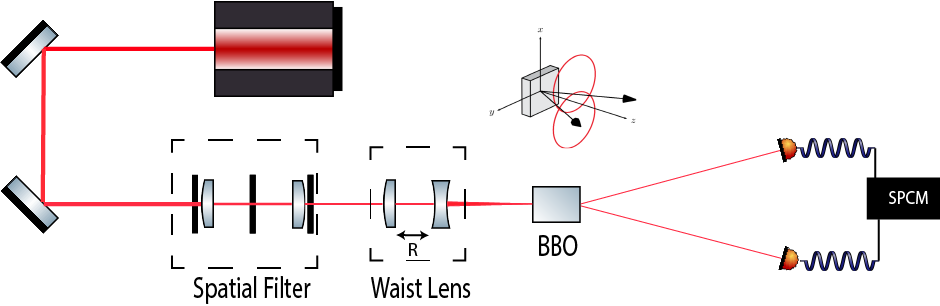
\includegraphics[width=0.8\textwidth]{Figures/SPDC.png}
\caption{Experimental Setup for the SPDC light Source} 
\label{fig:SPDC}
\end{figure}

\subsection{Diode Laser}
Before having pair of correlated photons, we start by having a coherent light source, 
for this experiment we use a Diode Laser that delivers a continuous wave(CW) at 
$\lambda = 406,101 nm$ and $\Delta \lambda = 4 nm$. 
The laser model No. DL 405-200 delivers light at 200 mW with a beam diameter 
of 1.5 mm and a beam Divergence\footnote{The beam divergence is an angular measure of the increase in beam diameter with distance from the original optical aperture}
 1.2 mrad. 

\begin{figure}[h!]
\centering
{  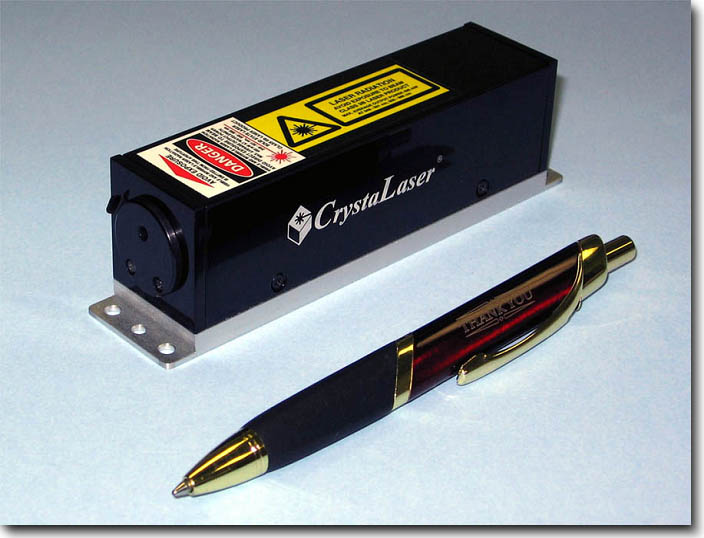
\includegraphics[width=0.45\textwidth]{Figures/diodeLaser.jpg} }
{  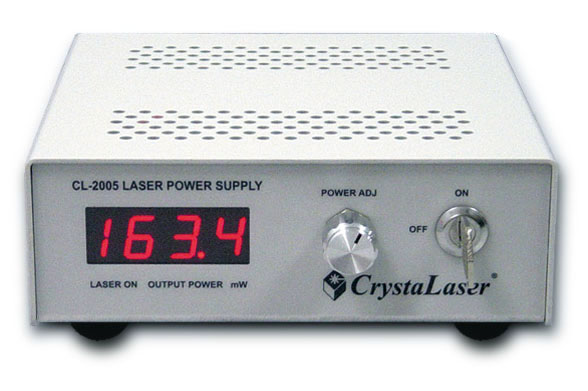
\includegraphics[width=0.45\textwidth]{Figures/diodeLaserControl.jpg} }
\caption{Image of the Diode Laser and it's control module, Taken from \cite{crystalLaser}}
 \label{fig:diodeLaser}
\end{figure}




\subsection{Mirror}
As seen in Figure \ref{fig:SPDC} we redirect the laser beam two times, for doing
so we use a pair of mirrors. For this kind of experiments, when the efficiency 
of the optical elements is really important, it is important to use the correct type
of mirror, we want a mirror that reflects most of the light. For this reason, depending
on the wavelength it is posible to find mirrors and lenses with different types of 
coating. Mirror and Lenses have a thin layer that is more efective for a range 
of wave lengths.

In Figure \ref{fig:mirror} we can see a Mirror and the base used to place it, it is posible
to manipulate the direction in which the mirror will reflect the light,  we can do this 
by manipulating the screws, each one moves the reflected laser in one direction. 
In the experimental setup we use two mirror to change the direction two times, this is because 
using just one could be more complicated when aligning the rest of optical elements. 
When two mirror are used, we have more possibilities, 4 in total. The advantage 
of having more possibilities is that the manipulation can be more precise.
\begin{figure}[h!]
\centering

 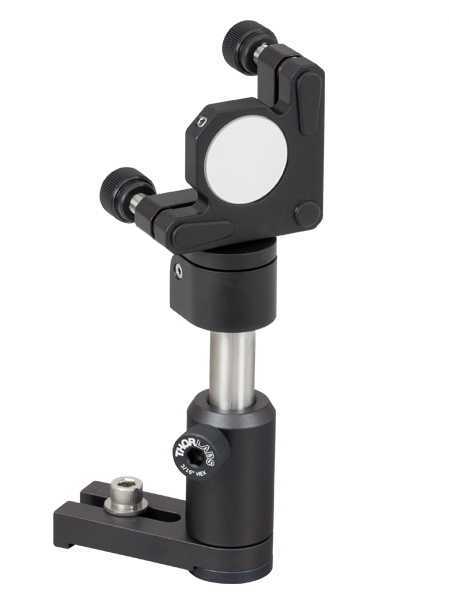
\includegraphics[width=0.3\textwidth]{Figures/mirror.jpg}
\caption{Mirror and the cavity mount} 
\label{fig:mirror}
\end{figure}

\subsection{Spatial Filter}
A laser beam can be characterized by measuring its spatial intensity profile at points perpendicular to its direction of propagation. 
The spatial intensity profile is the variation of intensity as a function of distance from the center of the beam, in a plane perpendicular to its direction of propagation.
\begin{figure}[h!]
\centering
{  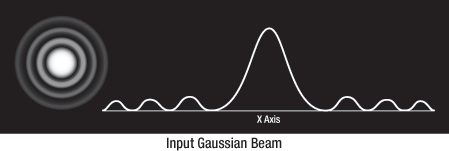
\includegraphics[width=0.6\textwidth]{Figures/inputBeam.png} }
{  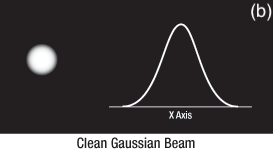
\includegraphics[width=0.6\textwidth]{Figures/outputBeam.png} }
\caption{The spatial intensity profile before and after the spatial filtering process , Taken from \cite{thorlabs}}
 \label{fig:inputOutputBeam}
\end{figure}
In Figure \ref{fig:inputOutputBeam} we se see the input gaussian beam 
and how its intensity fluctuates around the x axis. The output desired beam after going through the spatial filter is then shown.
The simplest arrangement to achieve this output spatial intensity profile is show in the Figure \ref{fig:spatialFilter}, 
where at the end we have a beam which intensity strength falls off transversely following a bell shaped curve that's symmetrical around the central axis.
\begin{figure}[h!]
\centering
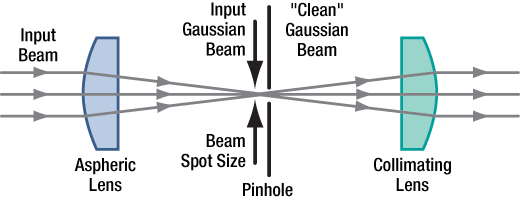
\includegraphics[width=0.55\textwidth]{Figures/spatialFilter.png}
\caption{Basic elements of a Spatial Filter. In our experiment we use a Aspheric Lens of $f=30 mm$(LA1805-A), a pinhole of $50 \mu m$ and a collimating lens of $f=60 mm$(LA1134-A). Taken from \cite{thorlabs}} 
\label{fig:spatialFilter}
\end{figure}
Taking a closer look at the input Gaussian beam in Figure \ref{fig:inputOutputBeam} we may recognise a diffraction pattern, the well known Airy disks. 
However, when we measure this spatial profile directly from the diode laser, we find out that it doesn't follow that behaviour, on the contrary 
it follows a more random spatial profile. This ramdom spatial profile is a result of the randomnes in the
quantum emissions and absorptions that are happening at the exited atoms at the diode laser\cite{hecht}.

In order to have this spatial intensity profile at the input of the lens arrangement, Figure \ref{fig:spatialFilter},
we put a circular aperture with the help of a iris, Figure \ref{fig:iris}, before the $f=30.0 mm$ lens. Another optional iris is placed after the $f=60.0mm$ lens.
\begin{figure}[h!]
\centering
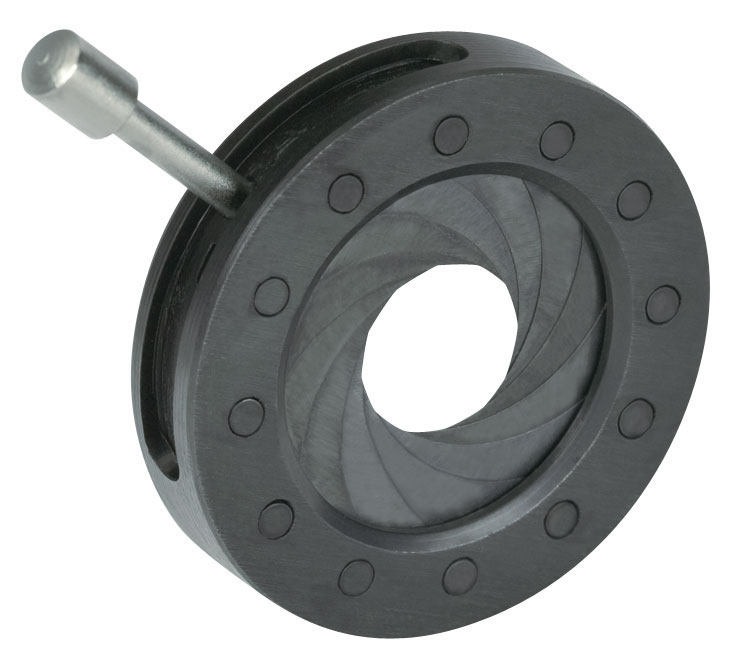
\includegraphics[width=0.25\textwidth]{Figures/iris.jpg}
\caption{This helps to form circular apertures of variable radius} 
\label{fig:iris}
\end{figure}


IN HERE I MAY TALK ABOU THE M FACTOR, QUALITY PARAMETER OF GAUSIAN BEAMS $M^2$ 
Power $200mW$

\subsection{Waist Lens}
After successfully achieving a Gaussian profile, which is important for the reasons described in Section \ref{sec:spatialCorrelations}.
After the spatial filter, we need a way to control the pump waist, but we need to do it in a way not too complicated, that 
doesn't imply too many changes in the experimental setup. Putting a  lens in the propagation direction with certain focal lenght $f$ will define a zone around
the distance f called \textit{Focus depth}\cite{hecht}, where in the middle we find the narrowest point of the beam.
The radius of this zone is:
\begin{equation}
 W_0=\frac{\lambda f}{\pi W_B}
\end{equation}
Where $W_B$ is the initial waist beam. 
In Figure \ref{fig:waist} we see this behaviour, this zone is produced around the distance $f$ and
the radius $W_0$ is a function of $f$ and $W_B$. making that if we want to change
$W_0$ we need to use a different lens with $f'$ and also the \textit{Focus depth}
will be at a different distance.

\begin{figure}[h!]
\centering
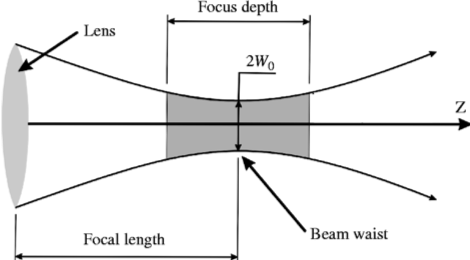
\includegraphics[width=0.35\textwidth]{Figures/waist.png}
\caption{Effect of lens on a Gaussian beam} 
\label{fig:waist}
\end{figure}

If we want to focus the beam at a fixed distance $F$, using this method to control the pump waist is not practical. 
Every different lens we would use will make this waist $W_0$ at a differents distances $f$. It is necessary to find a \textit{Waist lens}
that make us a $W_0$ at a transverse plane located in a fixed position $F$ from the \textit{Waist Lens}. 
In Figure \ref{fig:fixed} we present a special lens, consisting in an arrangment of two lenses, a positive 
and negative one respectively, separated a distance $d_0$ from each other.
\begin{figure}[h!]
\centering
 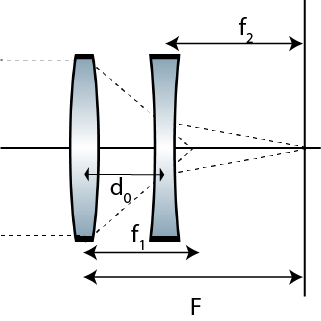
\includegraphics[width=0.65\textwidth]{Figures/fixed.png}
\caption{Composition of lenses to control the Pump Waist at a Fixed distance $F$} 
\label{fig:fixed}
\end{figure}
Where we can define a \textit{effective focal length} $F$ as a function of  $f_1$ and $f_2$, the focal lengths of the positive and negative lenses 
respectively. With the constrain that $d_0 < f_1$, $F$ reads:
\begin{equation}
F=\frac{f_1 |f_2|}{|f_2|-f_1+d_0}.
\end{equation}
This new effective focal length is crucial in the realisation of this experiment, as described before, we are interested in observing the effect 
in the reconstructed image using different spatial correlations. This is done by changing the pump waist of the laser that is focused on the crystal.
It is not experimentally practical to be changing the crystal position, it would mean to change the position of all the optical elements that 
follows. For this reason, it is perfect to be able to achieve the desired pump waist just by changing the relative separation of two lenses. 


\subsection{BBO(Beta Barium Borate) Crystal}
The Beta Barium Borate (BBO) is an inorganic compound, with chemical formula $\beta$-BaB$_{2}$O$_4$. This crystal is a
nonlinear optical media commonly used. It is also a birefringent\footnote{Birefringence is a optical property of some materials of 
having a refractive index that depends on the polarisation and the propagation of light\cite{hecht}} material and its transmission regions extends
from $189nm$ to $3500nm$\cite{bbo}.
The type-II crystal is mounted is such way that the input and output plane are fixed, Figure \ref{fig:bbo}(a). In particular the input plane is at $F$ from 
the \textit{waist lens} presented in the previous section, the power of the pump at this point is $\sim 60mW$. In Figure \ref{fig:bbo}(b) is a schem of 
the noncolinear configuration at the output plane of the crystal.

\begin{figure}[h!]
\centering
{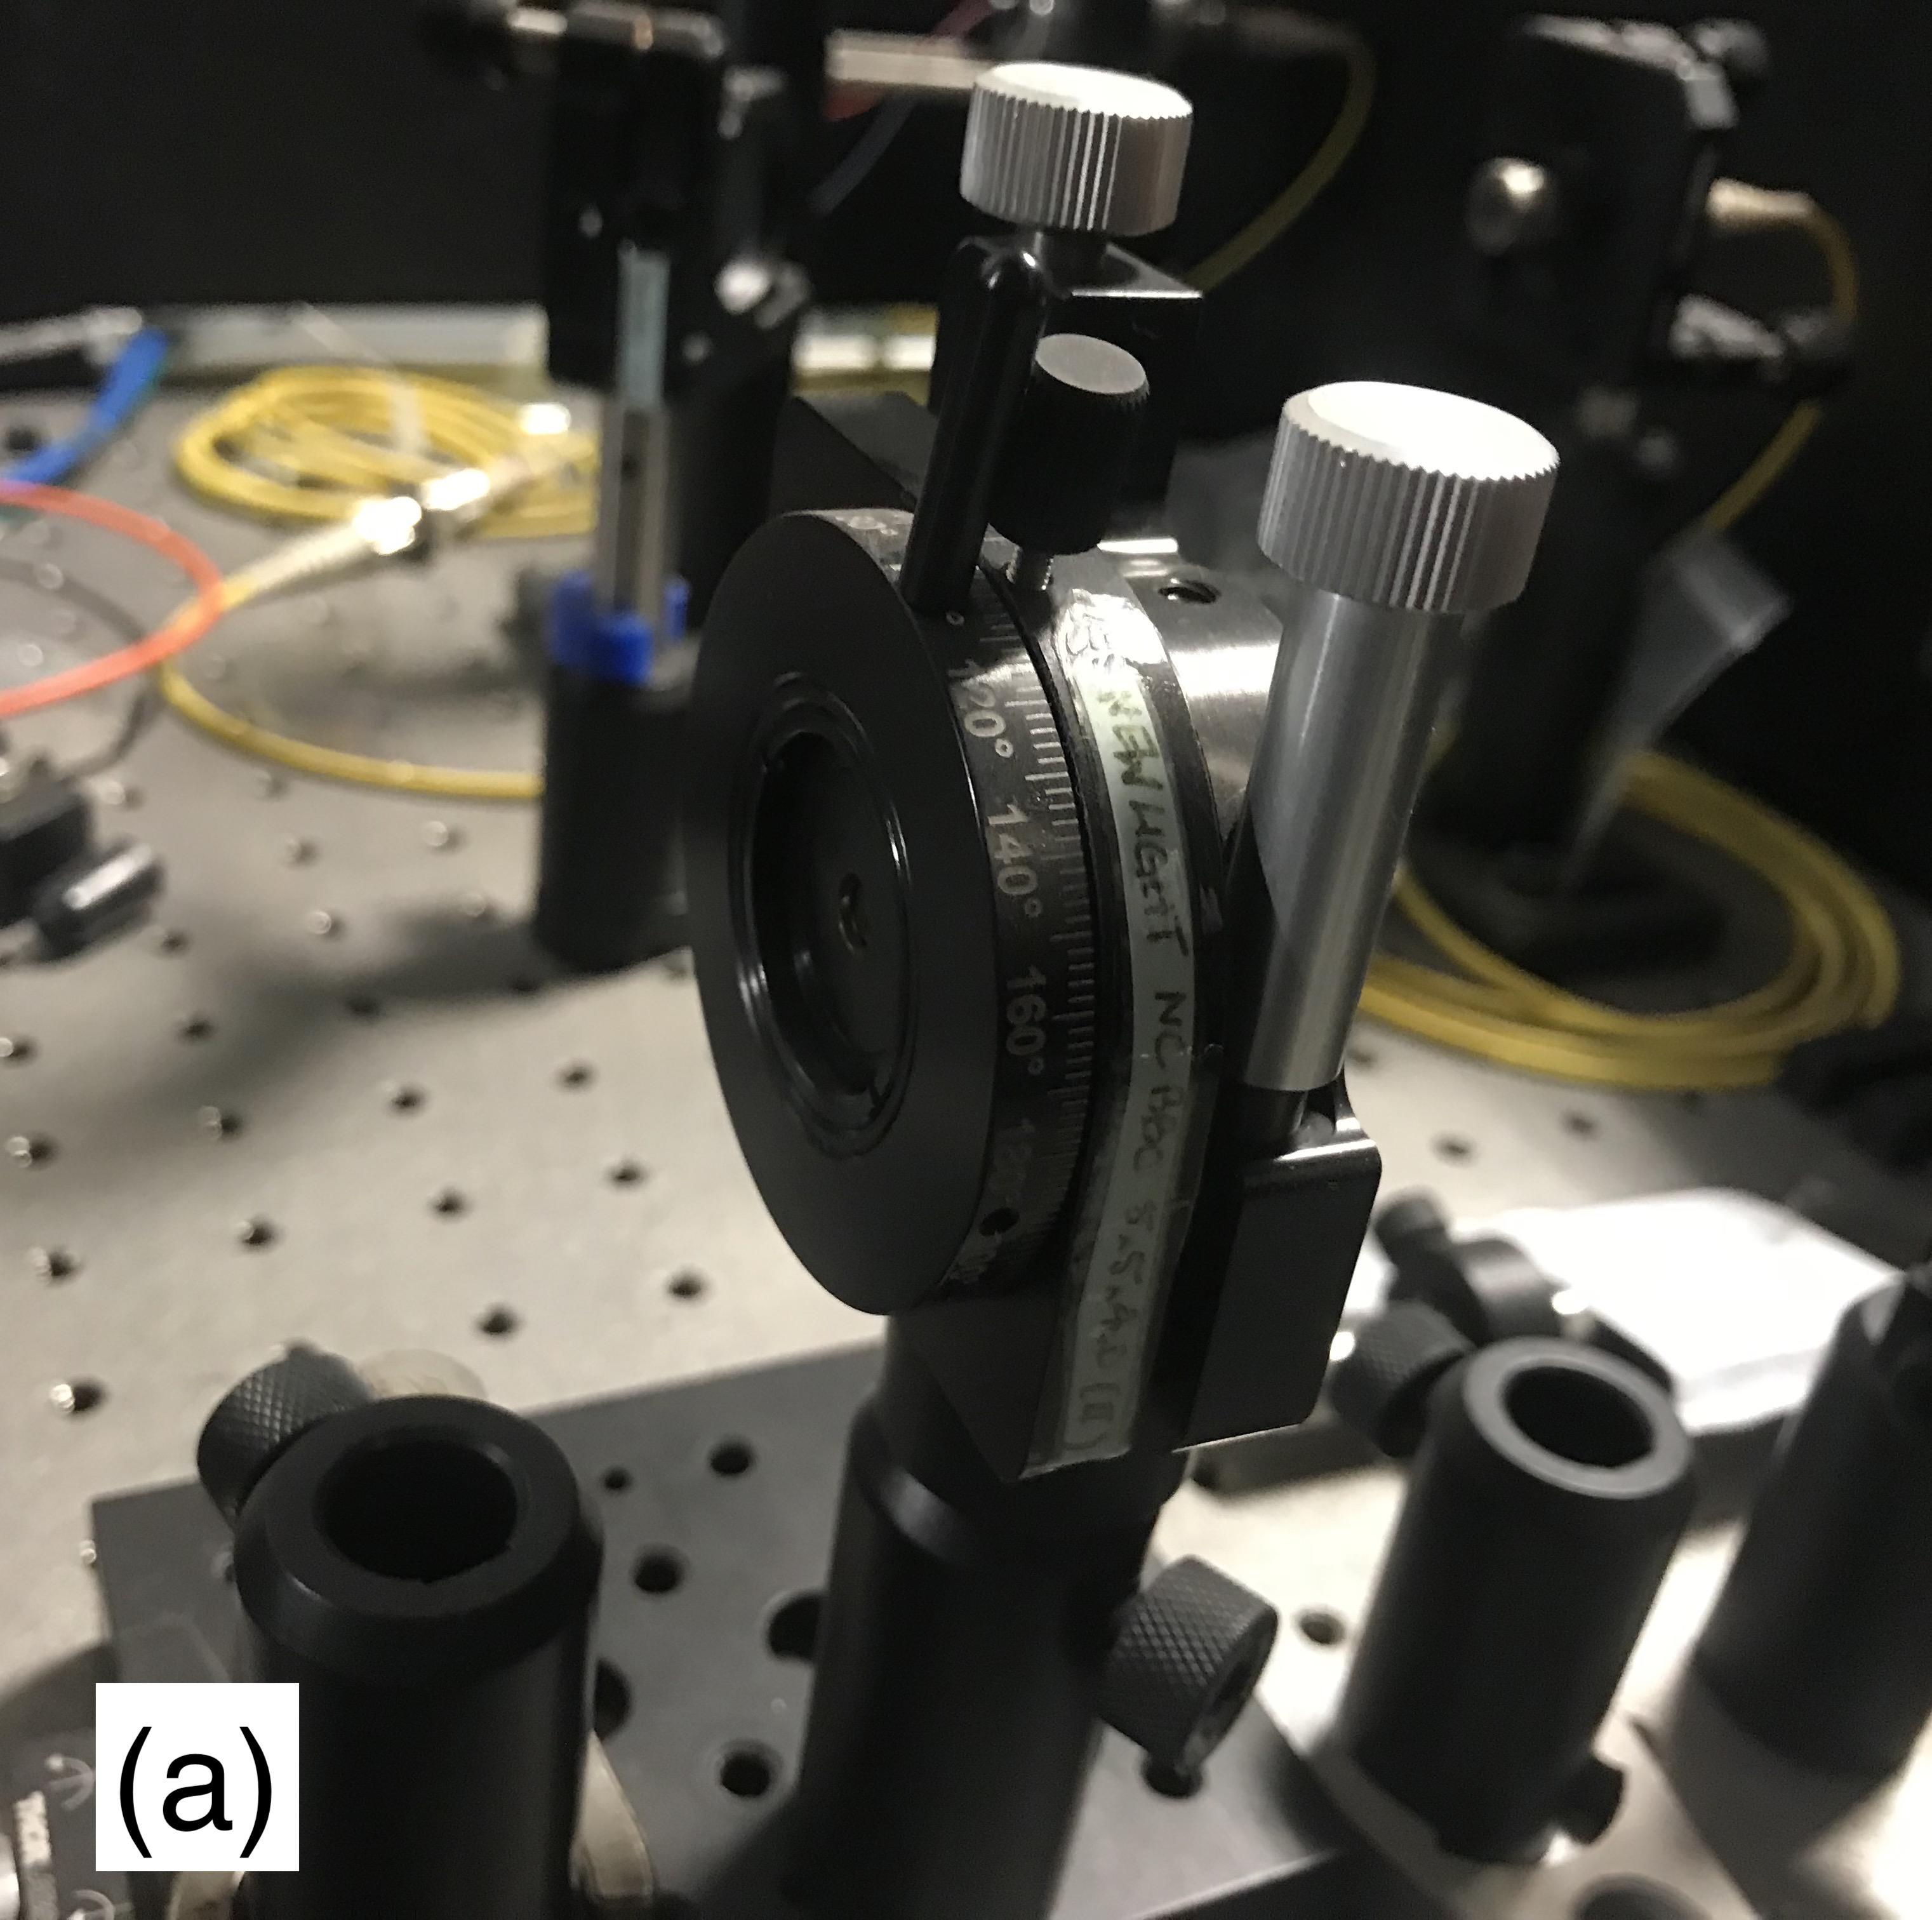
\includegraphics[width=0.35\textwidth]{Figures/bbo.jpg}}
{  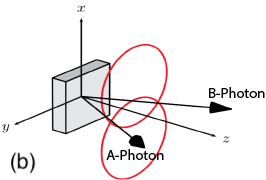
\includegraphics[width=0.5\textwidth]{Figures/aPhotonBPhoton.png} }
\caption{(a):Actual BBO crystal used in experiment. (b): the noncolinear configuration presented in this experiment}
 \label{fig:bbo}
\end{figure} 

At this point we have as a result of the SPDC process a pair of entangled photons, which have an strong correlation. This correlation is 
the feature in which we are interested on. We need to observe the shape of this correlations functions and the next section will focus 
on the experimental setup that will allow us to observe this.



\section{Spatial Correlations Measurement Setup}
From this point we will talk about a pair of correlated photons, that will come from the output plane of the BBO 
crystal, for historical reasons this photons are labeled as \textit{signal} and \textit{idler}. Nevertheless, to keep the same notations used through 
this monograph, this photon are going to be labeled as A-photon and B-photon, depending on which path they follow, in Figure \ref{fig:spatialSetup}
we can see the experimental setup for measuring the spatial correlations, and the different paths the light follows.

\begin{figure}[h!]
\centering
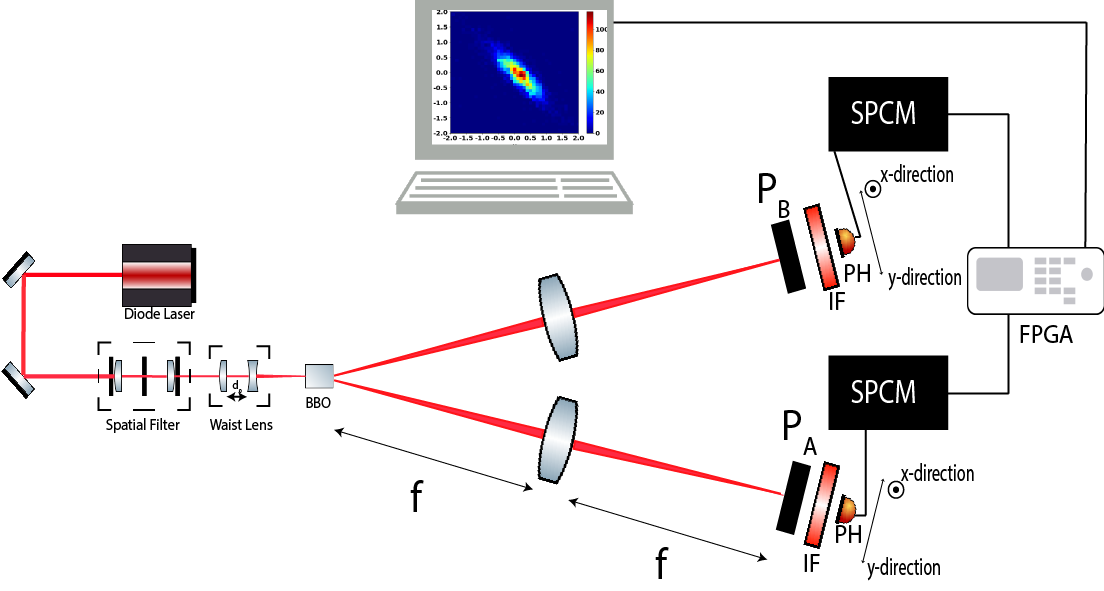
\includegraphics[width=1\textwidth]{Figures/spatialCorrelationSetup.png}
\caption{Experimental Setup for Obtaining the spatial correlations of a pair of down-converted photons} 
\label{fig:spatialSetup}
\end{figure}

\subsection{Lens (Fourier Plane)}
The next optical element that the pair of correlated photons find in their path is a pair of lenses. This pair of lenses are located at a
distance $f$ from the crystal. They define a $2f$ system and place a Fourier plane at a $2f$ distance from the crystal. As discused before, 
this plane is important because of the relation between the transverse momentum of the light before the 2-f system, and the photon 
position after de system, Eq. \ref{eq:fourier}. We use a lens(LA1708) of $f=200.0mm$ in front of each \textit{A} and \textit{B}. 


\subsection{Polariser}

We are interested in just a pair photons, $\Phi(\vec{q}_B,\Omega_B;\vec{q}_A,\Omega_A)$, that are polarised in certain direction. In order to filter the others
photons $\Phi(\vec{q}_A,\Omega_A;\vec{q}_B,\Omega_B)$, we place a pair of polarisers at both paths. A polariser is an optical element that filter light, it filters
light depending on the direction of the electrical field. We used a pair of Polarisers(WP25M-UB), which consist of an array of parallel metallic
wires sandwiched between glass with certain coating for better transmission.

\subsection{Interferometer Filter}
As pointed out in Section \ref{sec:spatialCorrelations}, in order to observe the transverse
correlations, the frequency information has to be traced out. For doing so, we placed a 
pair Interferometer filters. This optical elements have the special feature that only transmits 
light that comes throught in certain range of frequencies. To do this filtering we used a spectral filter(FB810-10) that only transmits the light that comes
with $\lambda =810 \pm 2nm$.

\subsection{Detection Module}
To observe the spatial correlations we have to be able to measure light that is propagating
in the z-direction. Figure \ref{fig:scan} shows the plane that is being scanned, where each 
square have a $x_i$ and $y_j$ position, ${i,j}$ goes from $0$ to $N$. With the help of a motorised translational stages, we can make this $N$ steps. we can 
control the movement of a pin hole detector, which consists in a single mode optical fiber tip. The translationas stages are controlled 
by Arduinos, this enable us to do the scan in a complete automated way.
\begin{figure}[h!]
\centering
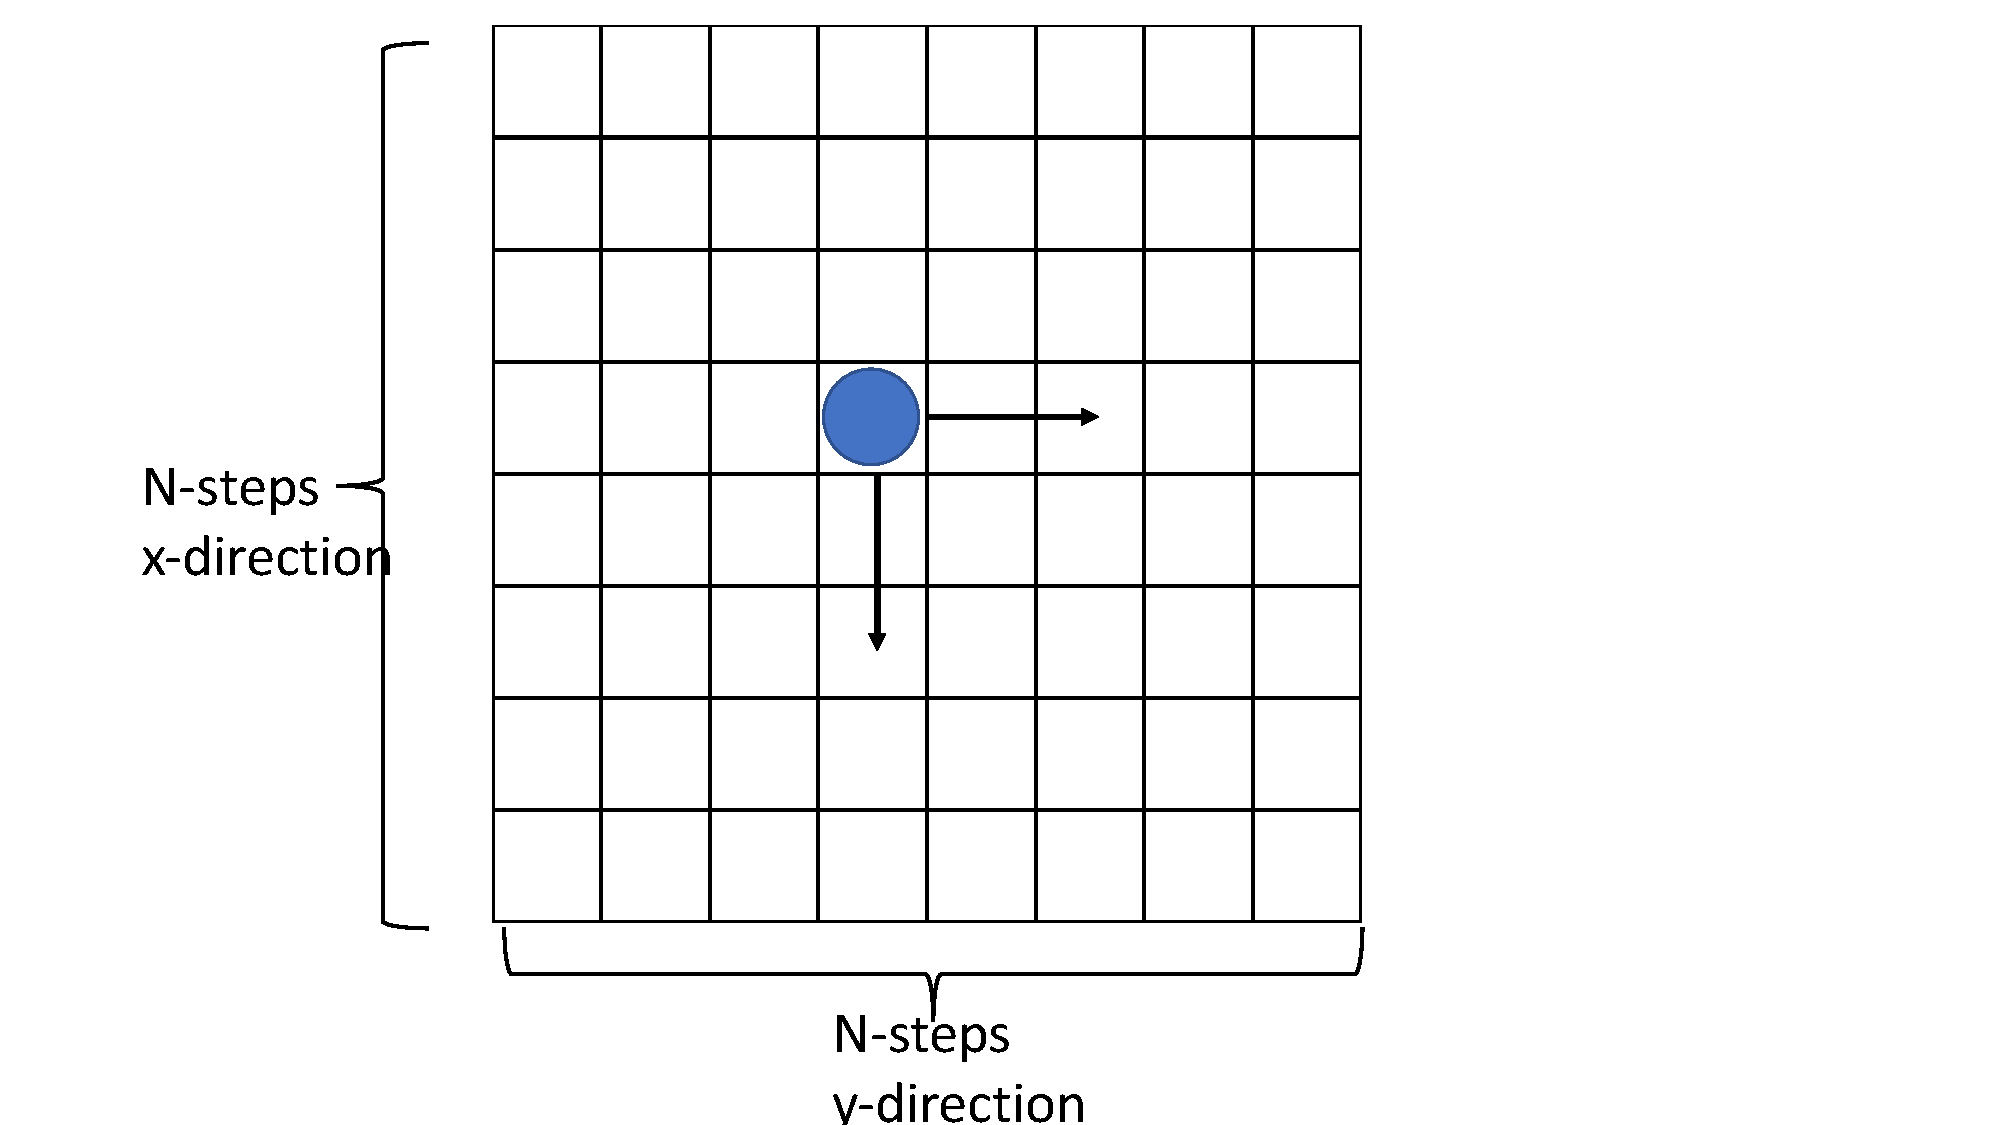
\includegraphics[width=1\textwidth]{Figures/scan.pdf}
\caption{The plane that is being scanned by the fiber tip, it is a $4x4mm$ square, that
can be scanned in N steps, where N is defined by us} 
\label{fig:scan}
\end{figure}

Another feature that is easily controlled, is the exposure time. It means we can set how many seconds, is going to be the fiber tip at
every ($i,j$) position. A greater time means more photon counted, and with a bigger amount of data of photons
counted per position, the means values per position gives a better image, with better contrast. The places where we don't have photons 
tend to have a low mean value of photons counted, while the more intense places keep counting, hence having bigger means values.
The ($i_B,j_B$) position and ($i_A,j_A$) position are related with $\vec{q}_B=(q_i,q_j)$ and $\vec{q}_A=(q_i,q_j)$ in Eq \ref{eq:quadratic} 
$\tilde{\Phi}(\vec{q}_B,\vec{q}_A)$, respectively. The spatial correlation we seek to observe. When taking a Two-photon imaging we already deduce in the 
previous Chapter that the image is going to be related with $R(\vec{r}_A)$ from Eq. \ref{eq:R}, where the ($i_A,j_A$)
 position is related with $\vec{r}_A=(x_i,y_j)$.






\subsection{Single Photon Counting Module(SPCM)}

Light is transmitted through an optic fiber from the pin hole detector to the SPCM. This 
consists in a self-contained module that detects single photons of light over the $400nm$ to $1069 nm$
wavelength range. The module used  is SPCM-AQRH-13, and it uses a unique silicon avalanche photodiode (SLiK) with a detection efficiency of more than 65\%\cite{spcm}.
The result signal coming from the SPCM are pulses where each one represents one photon.
\begin{figure}[h]
\centering
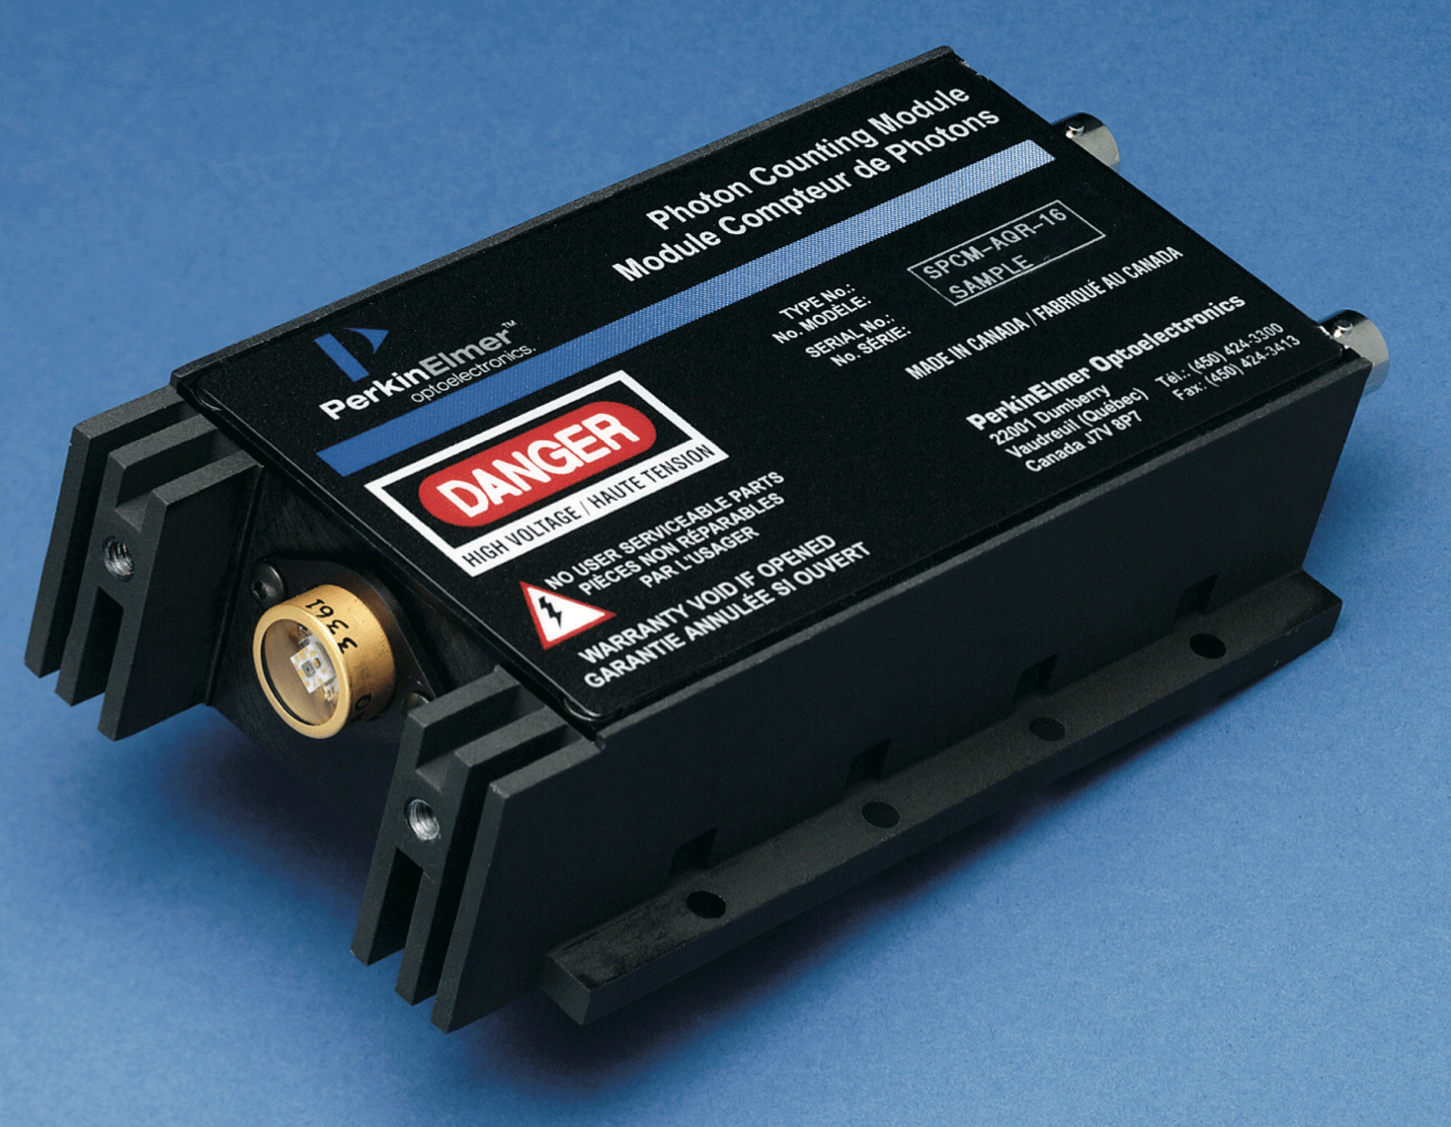
\includegraphics[width=0.35\textwidth]{Figures/spcm.png}
\caption{Single Photon Counting Module} 
\label{fig:spcm}
\end{figure}


\subsection{Field-programmable gate array(FPGA)}
Both \textit{A} and \textit{B} pulses from the respective SPCM goes to the same Field-Programmable Gate Array (FPGA). This
FPGA (ZestSC1) is programmed
to count the photon coincidences, this means that the FPGA is fast enough to detect and separate pulses from photons 
that are time-separated. 




\subsection{Computer(Data Analysis)}
LabvVIEW is used to control the detection module, and also, to recibe and translate the information
from the FPGA. It deliver the single and coincidence counts for every position in the 
scan grid, Fig. \ref{fig:scan}. Using this information is only matter of use any way to handle
this data and generate the graph for single and coincidence counts. Through this monograph
it has been used the python language and the matplotlib library to generate them.


\section{Two-Photon Imaging Setup}
For the Two-photon imaging process we no longer have spatial information about the  B-photon after it interacts
with the object. Figure \ref{fig:ghostSetup} shows the experimental setup for this stage of the
experiment. It is important to remember that all the setups shown so far, are in esence the same
optical elements, It was important to create a Experimental setup that allows us to 
measure different things without changing to much. In this stage we re-direct the light that 
goes through the object to a detector $D_C$.

\begin{figure}[h!]
\centering
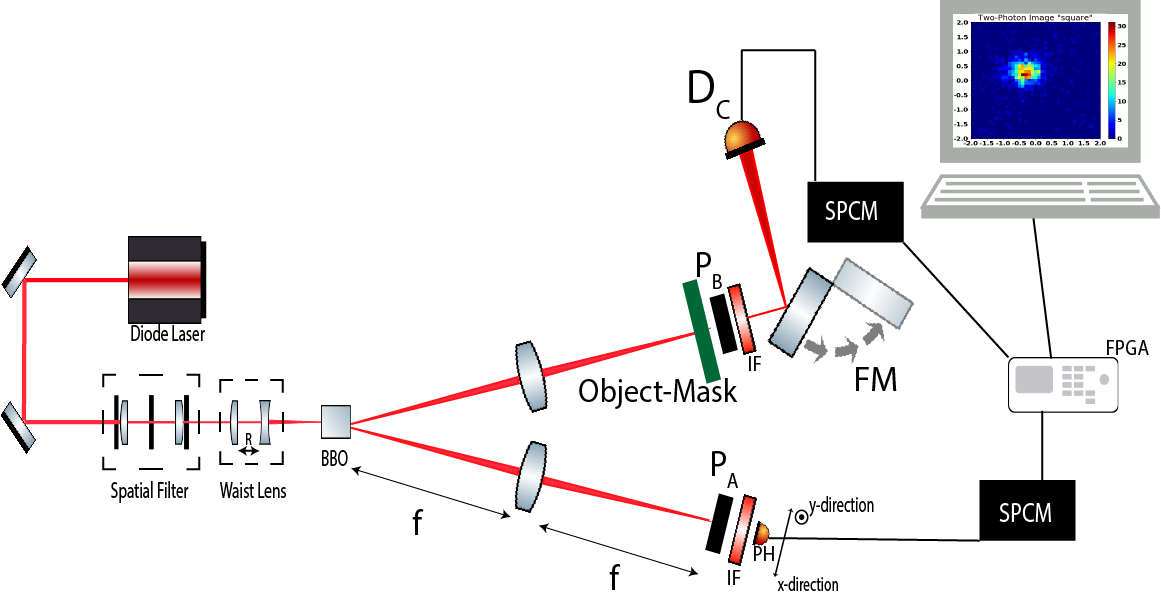
\includegraphics[width=1\textwidth]{Figures/ghostSetup2.png}
\caption{Experimental Setup for the Two-photon Imaging} 
\label{fig:ghostSetup}
\end{figure}

\subsection{Object-Mask}
This is an obstruction that is placed in the \textit{B} path. This is the object
from which we will make an image. It consist in an aperture on a translational mount,
that allow us to move the aperture precisely in the same plane we make our detections.
This is done by manipulating a pair of screws. 
We used differents objects and in Figure \ref{fig:mask1}
there is a detailed schematic of the first one used. It consists in a square aperture placed in the 4th 
quadrant of the scanned plane.

\begin{figure}[h!]
\centering
 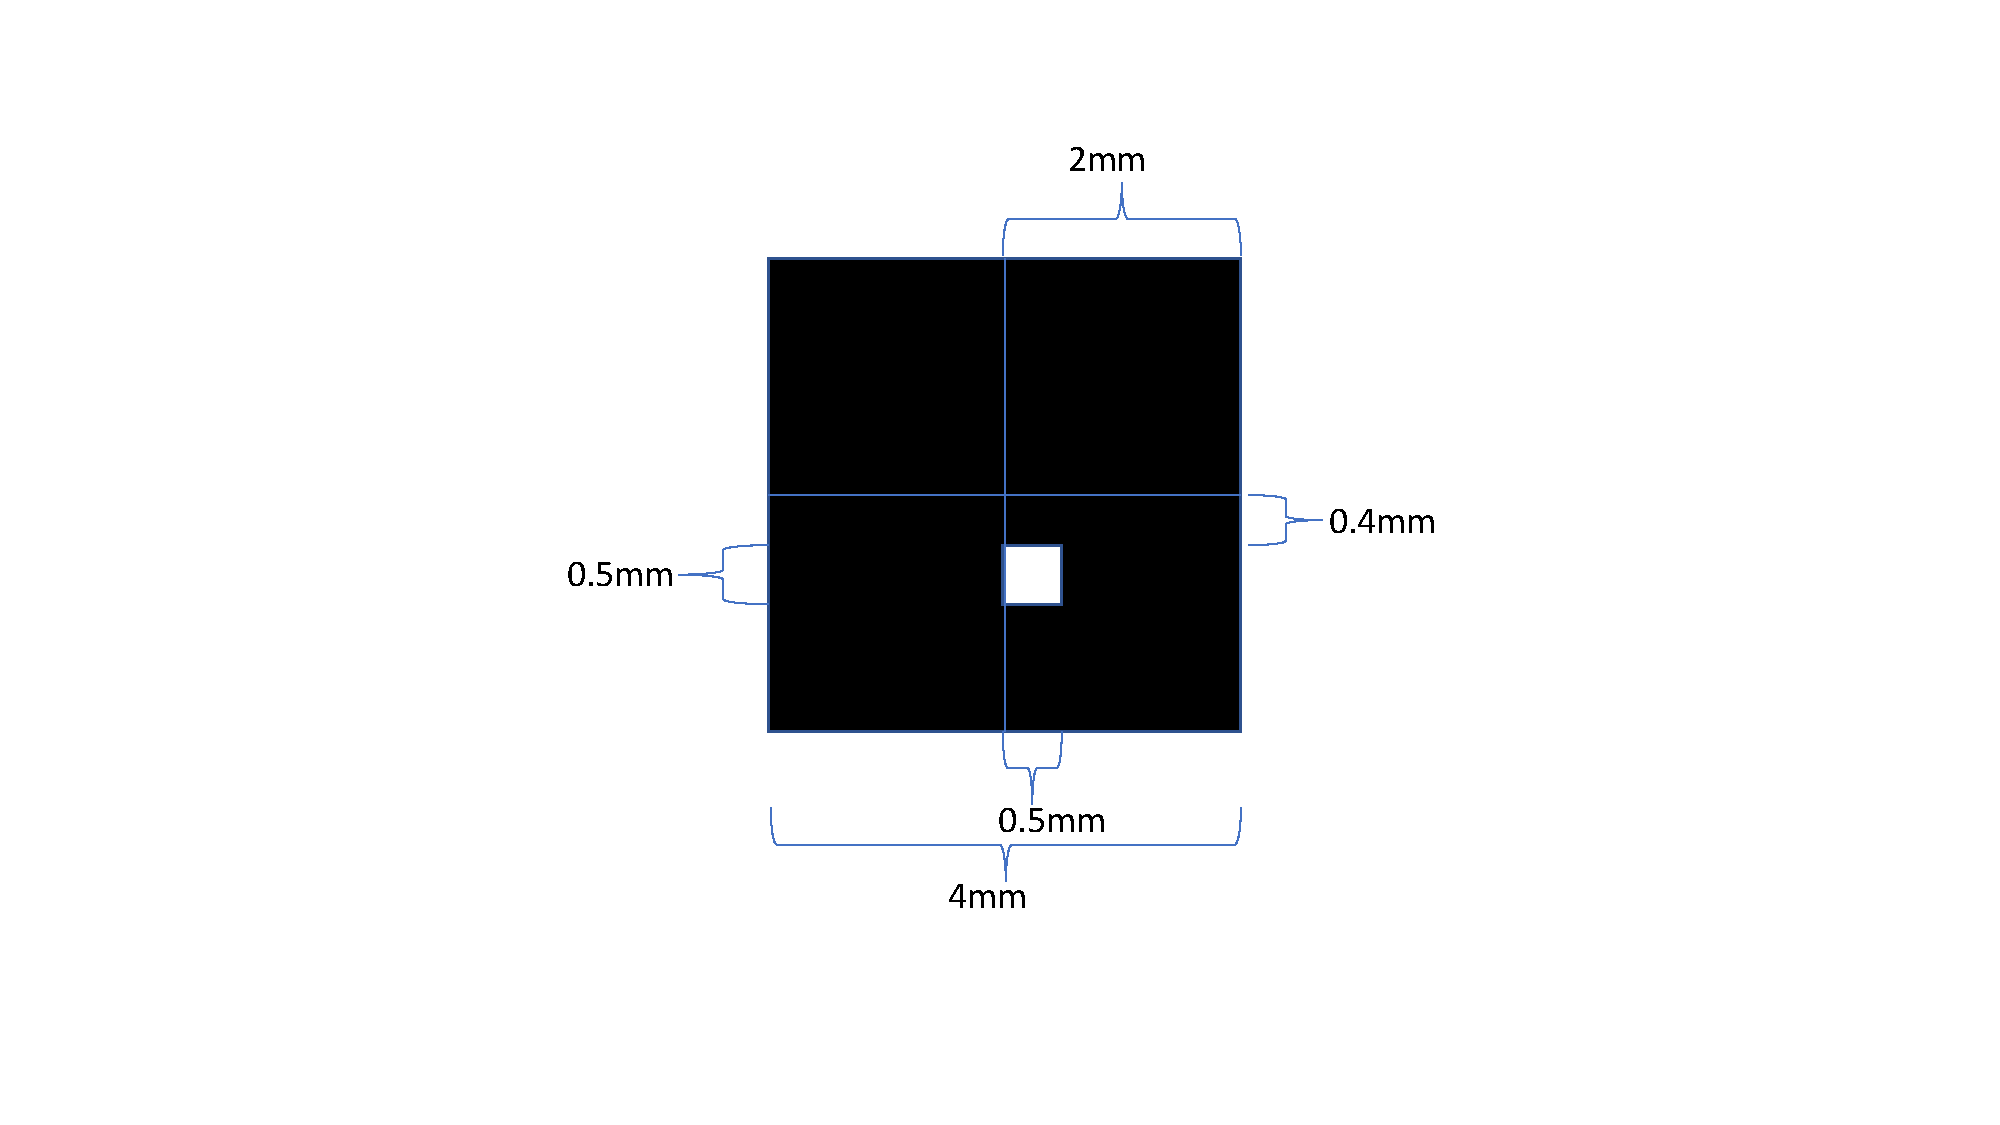
\includegraphics[width=0.6\textwidth]{Figures/mask1.pdf}
 \caption{Detailed description of the "square" aperture location in the scanned plane}
\label{fig:mask1} 
\end{figure}

In Figure \ref{fig:masks} there are the other two apertures that we used so far in the experiment, 
this apertures where selected because of the symmetries and antisymmetries they present, 
the goal of this monograh is to study the effect of the spatial correlations in the image
recovered, effect such as reflection of the original image, quality and others.  

\begin{figure}[h!]
\centering
{  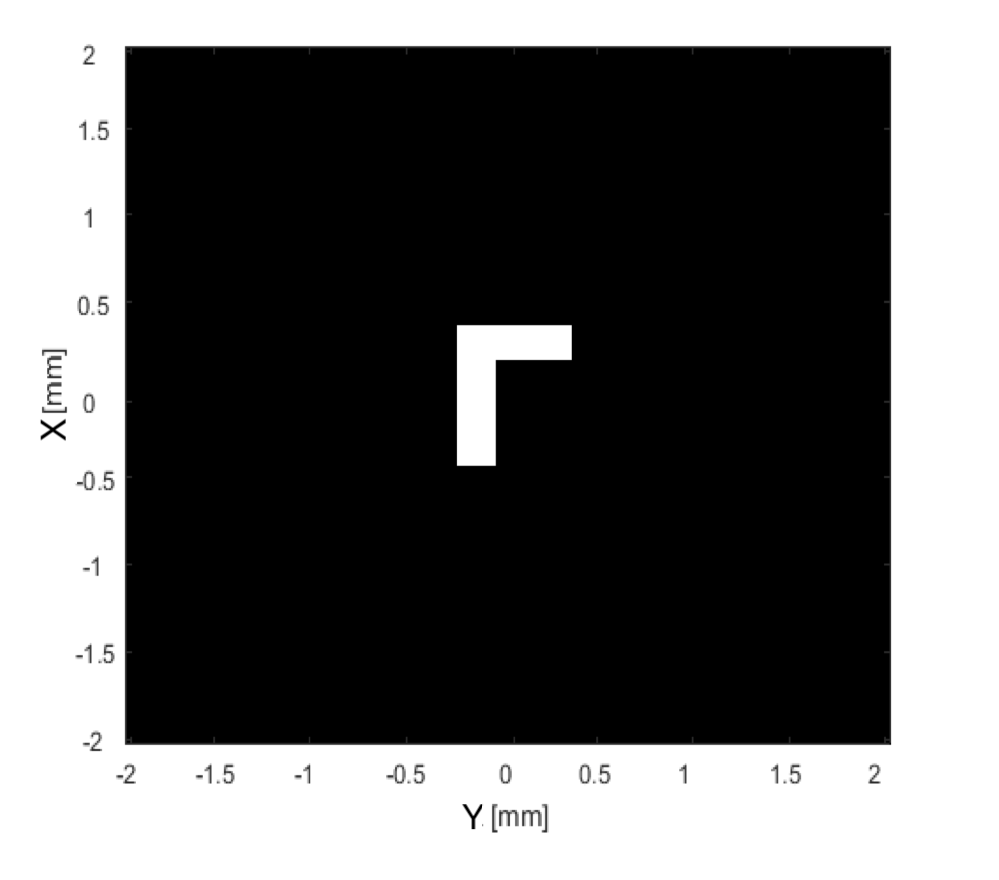
\includegraphics[width=0.45\textwidth]{Figures/mask2.png} }
{  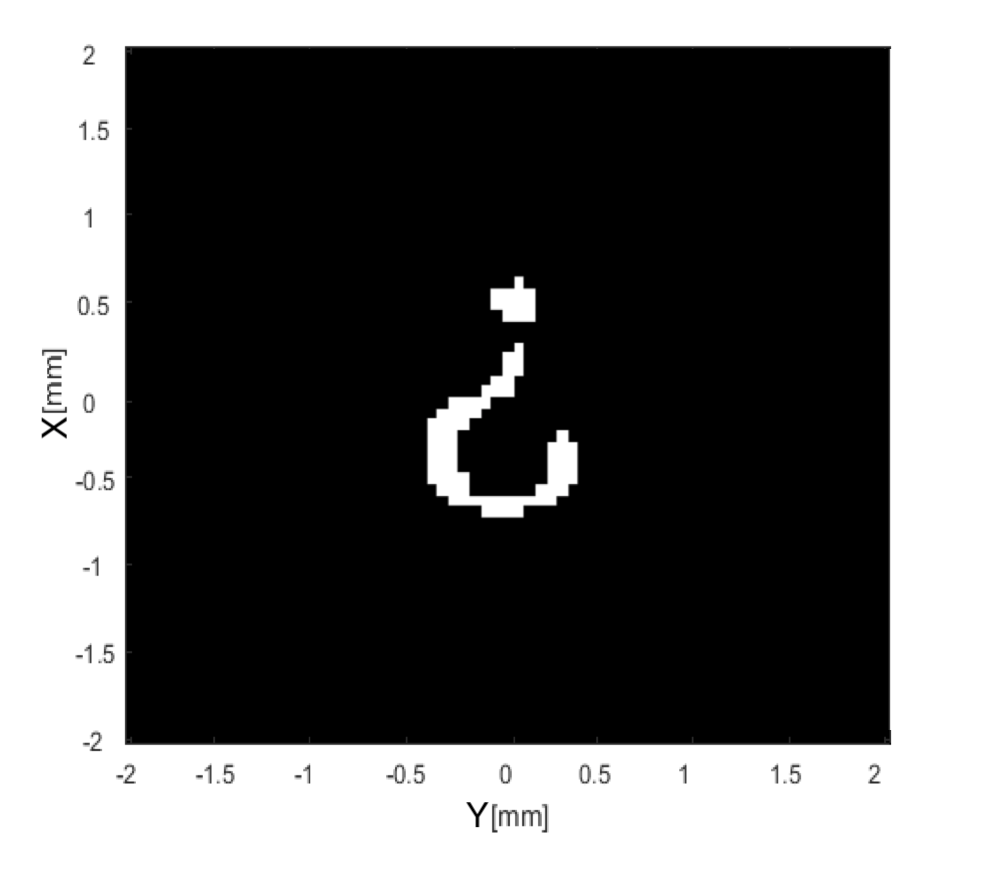
\includegraphics[width=0.45\textwidth]{Figures/mask3.png} }
\caption{The other two apertures used}
 \label{fig:masks}
\end{figure}

\subsection{Folding Mirror}
In order to change de path followed by the B-photon, and guide the light to a new detector $D_C$we use a Folding mirror, Figure \ref{fig:foldingMirror}.
This mirror plays the role of a switch, when is up, we are know dealing with the
$D_C$ detector, and we are doing a Two-photon Imaging process. In contrast, when the mirror is 
down, we are recovering spatial information, so it is possible to recognise some sort of
shadow from the object, or we are measuring the spatial correlations.
\begin{figure}[h!]
\centering
 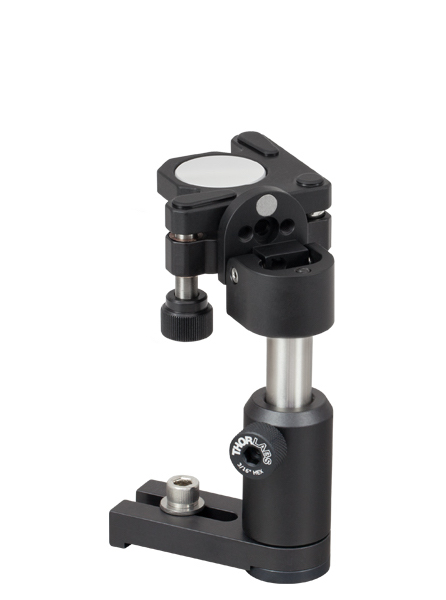
\includegraphics[width=0.25\textwidth]{Figures/foldingMirror.jpg}
 \caption{Foldind Mirror, it is in the position for measuring the correlations}
\label{fig:foldingMirror} 
\end{figure}

\subsection{Bucket Detector}
This detector consist denominated $D_C$ detector. It is a coupling lens that collects all the light that goes through the object.
The lens position is fixed, and it gathers all light and send it to a multi mode optical fiber connected to a SPCM.
In contrast to the other detections made before, the Bucket detector loses track of any spatial information of the photons. 